\documentclass[a4paper,12pt]{article}
\usepackage[utf8]{inputenc}
\usepackage[spanish]{babel}
\usepackage{color}
\usepackage{parskip}
\usepackage{graphicx}
\usepackage{multirow}
\usepackage{listings}
\usepackage{vmargin}
\graphicspath{ {imagenes/} }
\definecolor{mygreen}{rgb}{0,0.6,0}
\definecolor{lbcolor}{rgb}{0.9,0.9,0.9}
\usepackage{epstopdf}


\begin{document}

\title{Resumen de algunos de los virus más famosos de la historia}
\author{
Christofer Fabián Chávez Carazas \\
\small{Universidad Nacional de San Agustín} \\
\small{Seguridad Computacional}
}

\maketitle


\section{Storm BotNet}

Storm BotNet es una red de computadoras ``zombies'' contraladas remotamente e interconectadas por el gusano Storm.
Cuando un sistema es comprometido por este troyano, se propaga a si mismo enviando correos
electrónicos infectados con títulos provocativos como: ``Chinese missile shot down USA aircraft'' o
``U.S. Secretary of State Condoleezza Rice has kicked German Chancellor Angela Merkel.''\cite{storm}
Se estima que BotNet tenía un tamaño de aproximadamente 50 millones de computadoras \cite{storm}, lo vastante grande
como para verse implicado en varias actividades criminales, y lo suficientemente poderoso como para forzar paises enteros
fuera de la internet y superar a los más poderosos supercomputadores del mundo.  \par

Storm BotNet fue detectado por promera vez en Enero del 2007, llamado así por uno de los títulos que utilizaba en los correos
electrónicos que enviaba: ``230 dead as storm batters Europe''. Aún no se a identificado a los controladores de Storm BotNet.
Este botnet ha mostrado varios patrones defensivos que indican que los controladores protegen activamente el botnet, pero también
se ha visto que se protegía a si misma de ataques DDoS y atacaba los sistemas informáticos que analaizaban los sistemas infectados por
el gusano. También el gusano Storm ha intentado liberar miles de versiones de si mismo para poder dificultar la tarea de
las empresas de seguridad informática por convatir el virus.

En Octubre de 2007, Microsoft lanzó una actualización que eliminaba al gusano Storm de la máquina infectada. Esto ayudó a que
el tamaño del botnet se redujera considerablemente. En 2008, Storm botnet dejó de enviar spam, y con el paso de los años se fue eliminando
el gusano y reduciendo su tamaño. Hoy en día hay rumores de un Stormbot 2 basado en el código original de Storm botnet.



\section{ClickBot.a}

El ClickBot es un botnet que genera clicks automáticamente sobre la publicidad,
muy utilizado para burlar los sistemas pay-per-click(PTC) \cite{clickF}
Este BotNet cuenta con más de 100,000 computadoras bajo su control usando un HTTP-based botmaster.
Clickbot no se propaga automáticamente por sus propios medios, sino que precisa de la intervención de un usuario atacante para su propagación.
Los medios empleados son variados, e incluyen, entre otros, memorias USB, mensajes de correo electrónico con archivos
adjuntos, descargas de Internet, transferencia de archivos a través de FTP, canales IRC, redes de intercambio de archivos punto a punto (P2P), etc. \par
El ClickBot se registra como BHO (Browser Helper Object) para ejecutarse cada vez que Internet Explorer se ejecuta. Luego
Se registra en una base de datos del sistema de control. Después, espera hasta que recibe la orden de pulsar anuncios,
sobre qué anuncios debe pulsar y las palabras clave a las que va destinado. Y así el controlador consigue obtener beneficios econímicos
procedentes de los clicks fraudulentos.

\section{Stuxtnet}

Stuxnet es un gusano muy sofisticado diseñado para atacar sistemas de control y monitoreo de procesos (SCADA), empleando
vulnerabilidades de dia cero que tenía el sistema operativo Windows. Tambíen es uno de los primeros gusanos conocidos
que incluye un rootkit para sistemas reprogramables PLC. Stuxnet fue firmado digitalmente con dos certificados auténticos robados de autoridades de certificación. \cite{stux}\\
Stuxnet infecta una computadora inicial mediante memorias USB infectadas para luego contaminar otros equipos conectados a la red.
El objetivo más probable del gusano, según varios medios de comunicación, podría haber sido instalaciones nucleares en Iŕan.
Para ver una descripción general de Stuxnet vea la Figura \ref{fig:stux}. \par

\begin{figure}
 \centering
 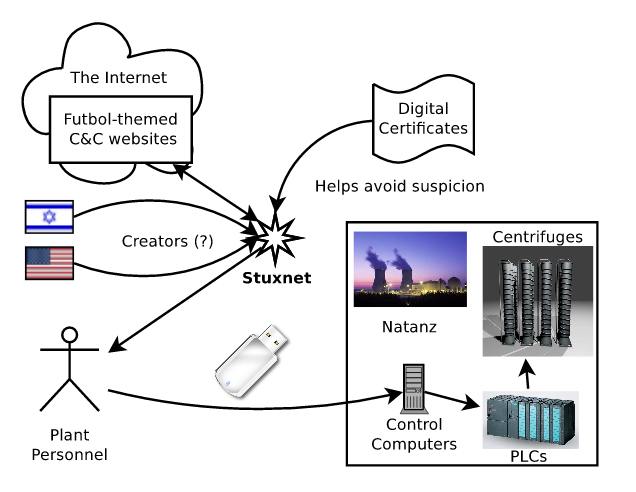
\includegraphics[scale=0.5]{stux.png}
 \caption{Visión general del Stuxnet \cite{stux}}
 \label{fig:stux}
\end{figure}

Stuxnet fue identificado primero por VirusBlockAda, una compañía de seguridad informática, a mediados de junio del 2010.
Una de las razones por la que los expertos creen que Stuxnet fue descubierto es que el virus se propagó accidentalmente mucho
más allá de su objetivo principal. Debido a un error en una actualización del gusano, el virus llegó a una computadora conectada
a internet, y así se hizo más público.

\section{Ransomware}

Es un tipo de virus que restringe el aceso a partes o archivos importantes dentro del sistema infectado, dejando así vía libre
para que el creador o controlador del ransomware pueda pedir algun tipo de rescate a cambio de quitar la restricción. Muchos
de estos programas maliciosos estan basados en la criptovirology, que estudia las formas de usar la criptografia para hacer dichos
programas mucho más poderosos. \cite{ran} \par

Existen cuatro tipos de ransomware. El ransomware por encriptación, que encripta la información de la víctima con llaves simétricas,
con la esperanza de que esta page para conseguir la llave y desencriptar la información. \\
El ransomware sin encriptación, que se aprobecha de otra forma de evitar que la víctima acceda a sus archivos, tales como mostrando
imágenes en el sistema.\\
El leakware, que es una forma inversa del ransomware, en lugar de pedir un rescate para recuperar el acceso a información,
el leakware roba información comprometedora de la víctima, y el atacante la extorciona con mostrar dicha información si es que
no se le paga.\\
El ransomware Mobile, simplemente un ransomware para dispositivos móbiles. \par

Existen ransomware muy famosos. Reventon bloqueaba totalmente el sistema de la víctima y mostranba mensajes que alegaban que 
la computadora había sido usada para actividades ilícitas, y que se había tomado poseción de su sistema. El virus pedía una fianza
para poder liberar el sistema. Para hacer todo esto creíble, Reventon mostraba la ip de la víctima e imágenes tomadas con
su cámara web. En la figura \ref{fig:ran} se puede ver el mensaje que se mostraba en una computadora infectada. \\

\begin{figure}
 \centering
 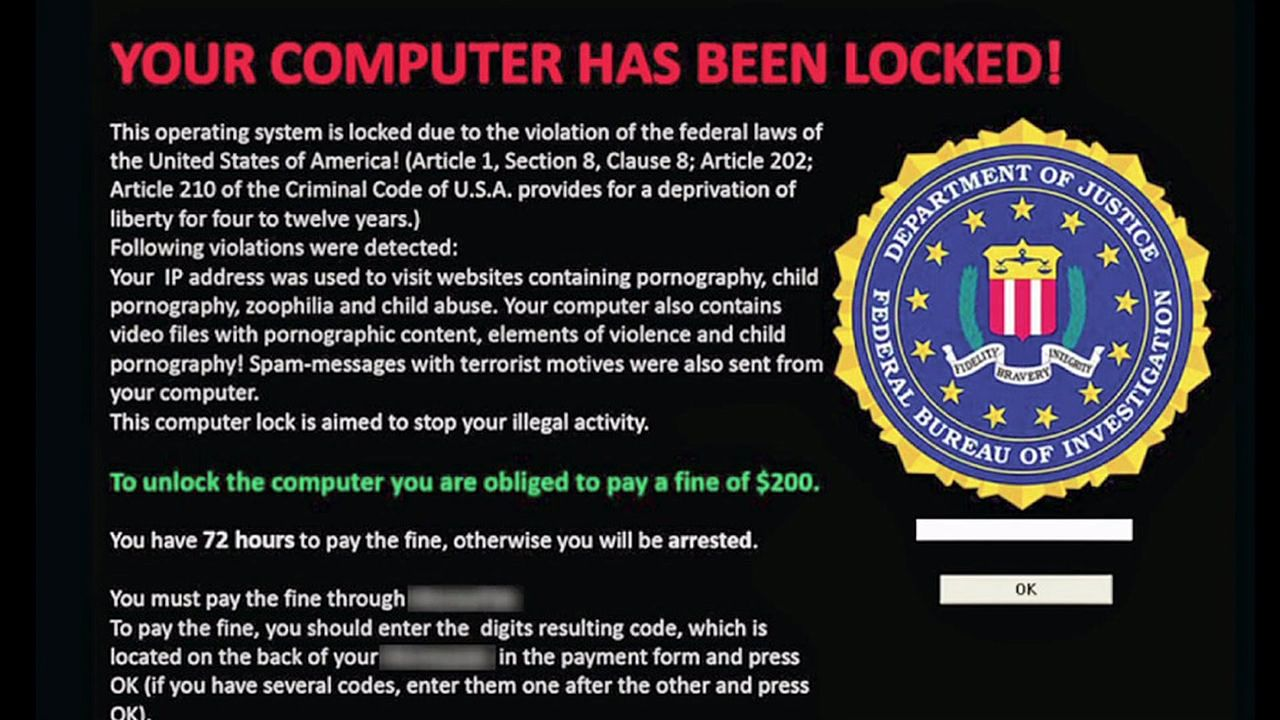
\includegraphics[scale=0.3]{ran.png}
 \caption{Mensaje mostrado por el Reventon}
 \label{fig:ran}
\end{figure}


CriptoLocker genera claves de 2048-bit del tipo RSA con la que se controla el servidor y se cifran archivos con una extención
específica. \\
Mamba es un nuevo ransomware de cifrado de disco completo que utiliza una estrategia de cifrado a nivel de disco
en lugar de uno basado en archivos convencionales. También sobrescribe el registro de inicio maestro del disco del
sistema que contiene el gestor de arranque para el sistema operativo. Esto prohíbe efectivamente al usuario de incluso cargar
el sistema operativo sin ingresar el código de descifrado, lo que supondría una nueva era para los ransomwares.


\begin{thebibliography}{X}
  \bibitem{storm} \textsc{Spiess, Kevin } \textit{Worm 'Storm' gathers strength. Neoseeker. September 7, 2007}  
  \bibitem{clickF} \textsc{Bernard J. Jansen} \textit{Click Fraud,  IEEE Computer. 40(7), 85-86.}
  \bibitem{stux} \textsc{Paul Mueller and Babak Yadegari} \textit{The Stuxnet Worm}
  \bibitem{ran} \textsc{Shafqat Mehmood} \textit{Enterprise Survival Guide for Ransomware Attacks. 3 May 2016}
\end{thebibliography}

\end{document}


